\procTitle{Анмангындинская наледь~--- индикатор изменения процессов водообмена криолитозоны Северо-Востока России}
\procAuthor{Землянскова~А.\,А., Нестерова~Н.\,В.}
\procEmail{anastasiazemlanskova@gmail.com}
\procOrganization{СВНИМС ИМЗ СО РАН} \procCity{Магадан}

\makeProcTitle
\index{z@Землянскова~А.\,А.}
\index{n@Нестерова~Н.\,В.}

Наледи~--- своеобразная форма сезонного оледенения, представляют собой крупные ледяные массивы в~долинах рек, регулирующие их водный и~ледовый режим.  Они являются показателем сложной взаимосвязи речных и~подземных вод в~условиях сурового климата и~многолетнемерзлых грунтов [5] и~играют существенную гидрологическую роль. Зимой наледи уменьшают речной и~подземный сток, а~в~тёплое время года талые воды наледей являются дополнительным источником питания рек.

Наледи дают информацию о запасе подземных вод, реагируют на изменение температуры воздуха и~количества осадков, а~также являются факторами формирования микроклимата и~являются индикаторами его изменения. В процессе фазового перехода вода~--- лёд~--- вода при образовании наледей и~их таянии в~тёплый период года вовлекаются огромные энергетические ресурсы. Энергия, которая выделяется и~поглощается, в~целом направлена на выравнивание температуры природной среды в~течение года, сезона, суток [4].

Для изучения многолетней изменчивости образования и~таяния наледей часто используют методы дистанционного зондирования Земли [3, 6]. На~основе космических снимков Landsat за период 2000--2019~гг. проведён анализ изменения площади Анмангындинской наледи. Межгодовая динамика не~показывает значимых изменений площади наледи. Анализ осложняется отсутствием снимков за одинаковые даты. В период весеннего половодья стаивает основная площадь наледи и~её изменение в~течение месяца может быть существенно (рис.~1).

\begin{figure}[h!]
\begin{changemargin}{-1.25cm}{0cm}
  \begin{center}
    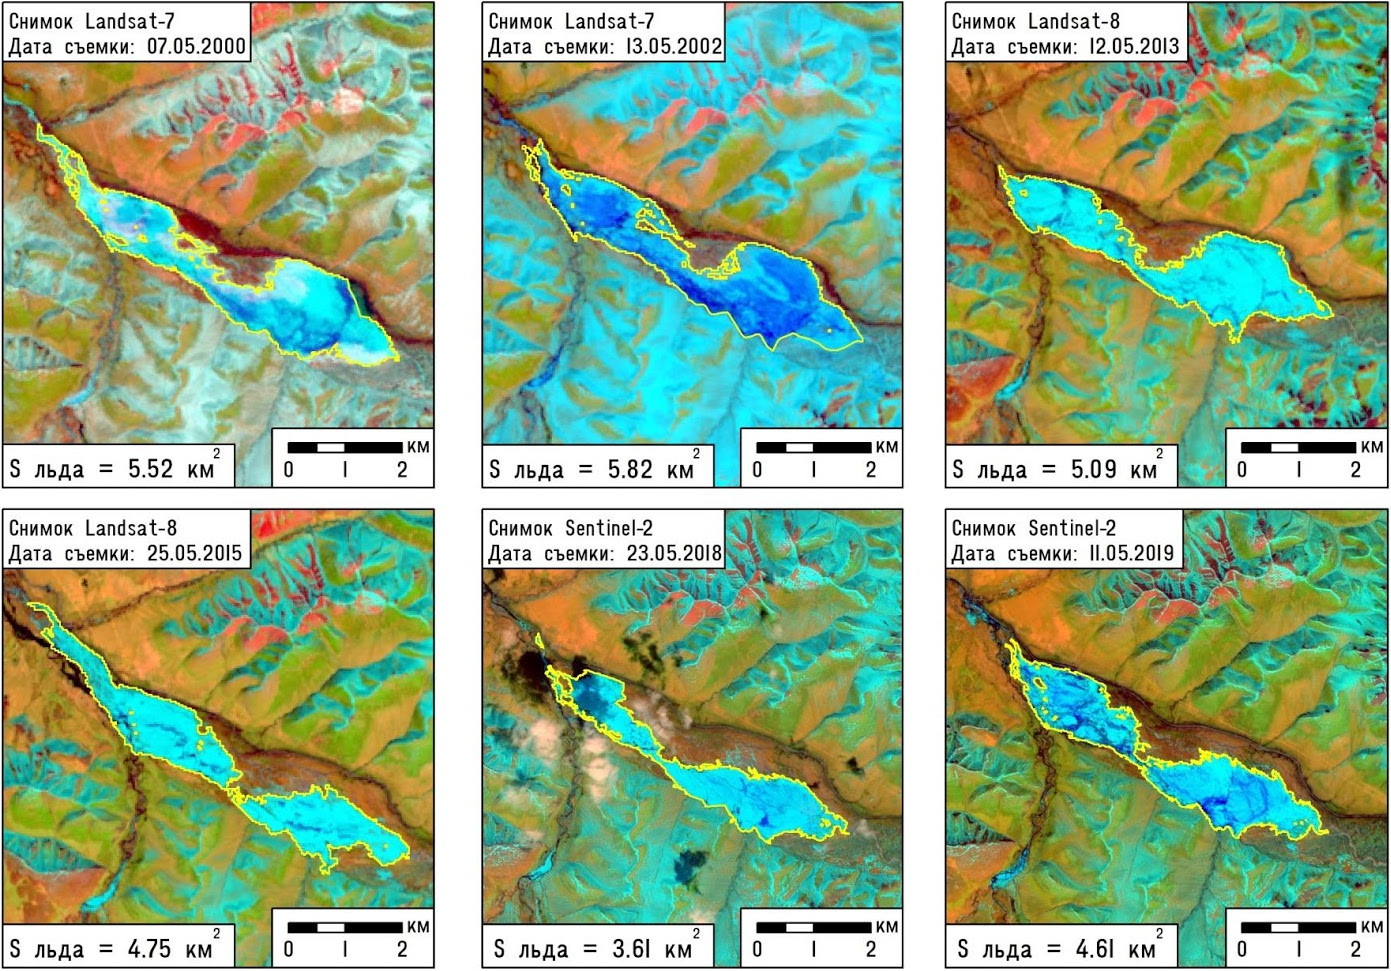
\includegraphics[width=1.2\textwidth]{authors/zemlaykova-1-fig-1.jpg}
  \end{center}
\end{changemargin}
  \caption{\textbf{Межгодовая изменчивость Анмангындинской наледи [2]}}
  \label{fig:zemlaykova-1-fig-1}
\end{figure}


Водосбор р.~Анмангында, в~котором образуется наледь, является репрезентативным для Северо-Востока России. Это единственный объект в~мире с продолжительным рядом наблюдений за процессами наледообразования, в~том числе динамикой площади и~объема наледного льда. Наледь расположена в~районе 155--159~км Тенькинской трассы (Магаданская обл.) в~30~км к~юго-востоку от пос.~Усть-Омчуг. Исследуемый водосбор находится в~пределах высот 700--1850~м и~относится к зоне сплошной многолетней мерзлоты, иногда прерывающейся в~таликовых зонах. Район исследования характеризуется суровой зимой и~коротким летом. По данным м/с~Усть-Омчуг средняя температура воздуха в~июле и~в~январе составляет +10,7\,\dgС и~$-$27,7\,\dgС соответственно (1966--2012~гг.), а~годовая сумма осадков~--- в~среднем 375~мм. Мощность многолетнемерзлых пород достигает 200 м, прослеживается увеличение на водораздельных участках и~снижается в~речных долинах [2].

Колымским УГМС 1962--1992~гг. были организованы стационарные наблюдения на Анмангындинской наледи. Работы включали изучение динамики роста и~таяния наледного тела, влияние климатических факторов на~процессы образования, роста и~разрушения наледи, измерение стока с~бассейна. За время наблюдений объем гигантской Анмангындинской наледи сократился вдвое. Такие изменения обусловлены повышением температуры воздуха и~количества атмосферных осадков [1].

Летом 2020~г. авторским коллективом при поддержке РГО и~РФФИ и~содействии руководства Института Мерзлотоведения им.~П.\,И.~Мельникова СО РАН в~течении двух недель было проведено рекогносцировочное обследование Анмангындинской наледи на предмет возможности проведения научных работ и~восстановления стационарного мониторинга состояния мерзлоты и~гидрологических процессов.

За период 4--19 июля 2020~г. дана оценка вклада наледного стока в~питании реки Анмангында, рассчитан коэффициент стаивания, проведён гидрохимический и~изотопный анализ проб воды. Для оценки мерзлотно-гидрогеологический условий выполнено ландшафтное профилирование наледной поляны, особое внимание уделено описанию растительного покрова, свойств горных пород, слагающих наледную поляну и~геокриологическим явлениям. Использование современного оборудования, такого как беспилотный летательный аппарат (БПЛА) позволило составить подробный ортофотоплан наледной поляны, а~также проследить изменение площади наледи за короткий промежуток времени. Так, с 4 по 15 июля произошло сокращение площади наледного льда в~два раза с 0,65~км$^2$ до 0,31~км$^2$. По данным нивелирной съёмки рассчитаны величина и~скорость стаивания на репрезентативных площадках, максимальные значения которых за период с 10 по 18 июля составили 68,6~см и~7,7~см/сут. соответственно (рис.~2). Коэффициент стаивания, рассчитанный на основе скорости таяния и~сумме среднесуточных температур, максимально составил 4,57~мм/(\dgС$\cdot$сут.).

\begin{figure}[h!]
  \begin{center}
    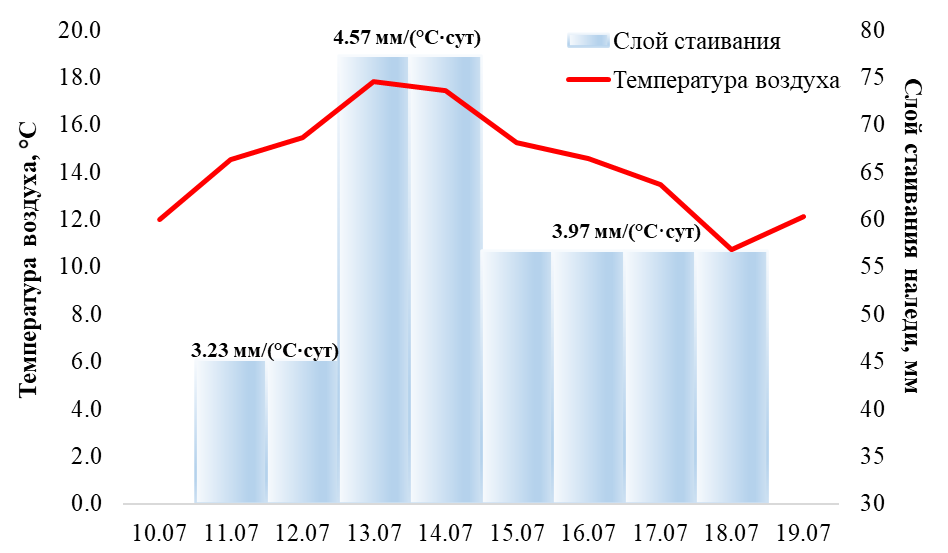
\includegraphics[width=0.8\textwidth]{authors/zemlaykova-1-fig-2.png}
  \end{center}
  \caption{\textbf{Оценка скорости стаивания наледи по результатам нивелирной съёмки}}
  \label{fig:zemlaykova-1-fig-2}
\end{figure}


По первому этапу работ получена оценка водного баланса р.~Анмангында с учетом наледного стока, который составил 3,2\,\%. Для этого было организовано три гидрологических поста, на которых ежедневно измерялись расходы воды, с помощью логгеров получены часовые данные об уровне и~температуре воды; установлена метеостанция и~осадкомер, регистрирующие часовые данные температуры воздуха, давления и~количества осадков. с увеличением температуры воздуха увеличивается и~скорость таяния льда.

Продолжение режимных наблюдений на Анмангындинской наледи и~сравнение их с историческими данными позволит изучить динамику наледеобразующих источников и~оценить интенсивность и~трансформацию водообменных процессов при изменении природной среды и~климата.

Исследования проводятся при поддержке РФФИ~--- проекты №~20-05-00666~А, №~19-55-80028, и~Русского Географического Общества~--- проект <<Атлас гигантских наледей-тарынов Северо-Востока России>>.

\begin{thebibliography}{99}
\bibitem{}\BibAuthor{Алексеев~В.~Р.} Многолетняя изменчивость родниковых наледей-тарынов // Лед и~снег.~--- 2016.~--- Т.~56, №~1.~--- С.~73--92.
\bibitem{}\BibAuthor{Букаев~Н.} Основные закономерности режима гигантских наледей в~верховьях р.~Колыма (на примере Анмангындинской наледи) // Колыма.~--- 1966.~--- №~4.~--- С.~9--12
\bibitem{}\BibAuthor{Макарьева~О.~М., Шихов~А.~Н., Осташов~А.~А., Нестерова~Н.~В.} Наледи бассейна р.~Индигирка по современным снимкам Landsat и~историческим данным c~2019~г. // Лёд и~Снег.~--- 2019.~--- №~59~(2).~--- С.~201--212.~--- DOI:~10.15356/2076-6734-2019-2-388.
\bibitem{}\BibAuthor{Поморцев~О.~А., Кашкаров~Е.~П., Попов~В.~Ф.} Наледи: глобальное потепление климата и~процессы наледеобразования (ритмическая основа долгосрочного прогноза) // Вест. Якутского гос. ун-та.~--- 2010.~--- Т.~7, №~2.~--- С.~40--48.
\bibitem{}\BibAuthor{Соколов~Б.~Л.} Наледи и~речной сток.~--- Л.~: Гидрометеоиздат, 1975.~--- 190~с
\bibitem{}\BibAuthor{Makarieva~O., Shikhov~A., Nesterova~N., Ostashov~A.} Historical and recent aufeis in the Indigirka River basin (Russia) // Earth Syst. Sci. Data.~--- Vol.~11.~--- P.~409--420.~--- DOI:~10.5194/essd-11-409-2019.
\end{thebibliography}
